
\subsection{PARTICLE IMAGE VELOCIMETRY}

$PIV$ is a technique to determine the  velocity field of objects from a stream of images\cite{Bastiaans}.
The result of the $PIV$ is given as a vector field, showing for each particle, direction, sense and intensity of velocity. 
Moreover, the $PIV$ can be used for track different objects in the same image.
For this purpose, the $PIV$ technique divides a frame, by example the frame 1, in many possibles regions where targets can be found; 
to this purpose, each region of frame 1 and 2 are correlated using comparative method, 
so that a vector or a field of vector is generated 
starting of initial point till final point. Thus, we have displacement and the acquisition time between frames, 
so that applying derivate concepts it is possible to estimate the relative velocity.

\begin{figure}[H]
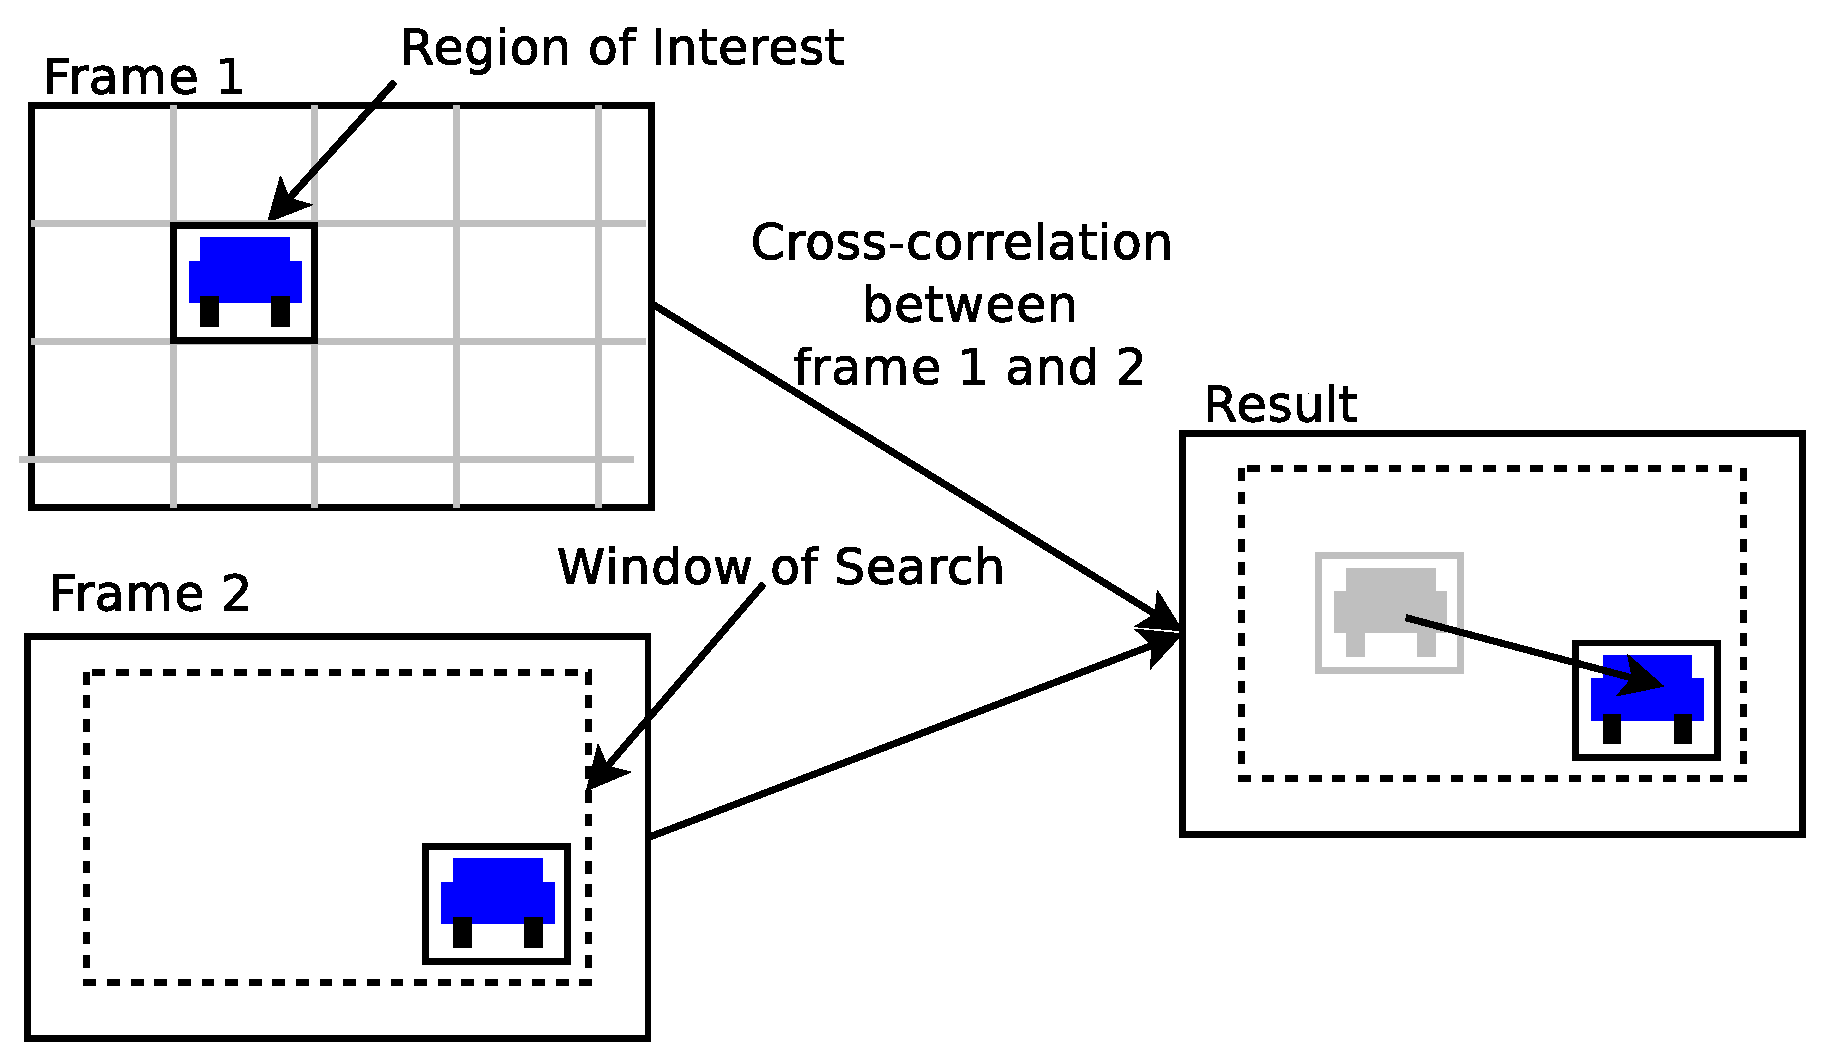
\includegraphics[width=\columnwidth]{images/explanationPIV.eps}
\caption{The PIV operation comparing two frames}
\label{fig:twoframes}
\end{figure}

The Fig. \ref{fig:twoframes} illustrates how $PIV$ works and demonstrates the relation between Region of Interest ($ROI$) and 
Window of Search ($WOS$). where $WOS$ is a region where the target will be searched and consequently $WOS$ must involve ROI. 
$WOS$ doesn't fill necessary whole image. If $WOS$ is large, we have an augment of computing but 
if $WOS$ is too small, target in high velocity has more chances to be lost. In our application, 
we determine $WOS$ from $1.5$ of $ROI$. For example, if ROI is $200\times300$ so we have WOS of $300\times450$. 
This consideration can be tuned by tests, by example considering environments with objects
of low velocity (permitted velocity in cities and roads).

\begin{figure}[H]
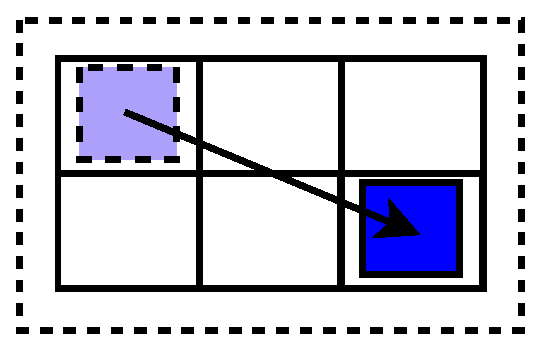
\includegraphics[width=\columnwidth]{images/WOSdivided.eps}
\caption{The $ROI$ is searched in the $ROI$ on windows of same dimensions. }
\label{fig:WOSdivided}
\end{figure}

$ROI$ is one of most important part of $PIV$, because it contains target. An Analysis Region ($AR$)
of same dimension of $ROI$ is displaced
along of whole $WOS$ in frame $2$, like showed in Fig. \ref{fig:WOSdivided}. Comparisons are done among regions between frames and are 
assigned values. 
When process finishes, the more height value refers the new place of $ROI$. It means that target displaced of a point in 
frame $1$ to another in frame $2$.